% Options for packages loaded elsewhere
\PassOptionsToPackage{unicode}{hyperref}
\PassOptionsToPackage{hyphens}{url}
%
\documentclass[
]{article}
\usepackage{amsmath,amssymb}
\usepackage{lmodern}
\usepackage{iftex}
\ifPDFTeX
  \usepackage[T1]{fontenc}
  \usepackage[utf8]{inputenc}
  \usepackage{textcomp} % provide euro and other symbols
\else % if luatex or xetex
  \usepackage{unicode-math}
  \defaultfontfeatures{Scale=MatchLowercase}
  \defaultfontfeatures[\rmfamily]{Ligatures=TeX,Scale=1}
\fi
% Use upquote if available, for straight quotes in verbatim environments
\IfFileExists{upquote.sty}{\usepackage{upquote}}{}
\IfFileExists{microtype.sty}{% use microtype if available
  \usepackage[]{microtype}
  \UseMicrotypeSet[protrusion]{basicmath} % disable protrusion for tt fonts
}{}
\makeatletter
\@ifundefined{KOMAClassName}{% if non-KOMA class
  \IfFileExists{parskip.sty}{%
    \usepackage{parskip}
  }{% else
    \setlength{\parindent}{0pt}
    \setlength{\parskip}{6pt plus 2pt minus 1pt}}
}{% if KOMA class
  \KOMAoptions{parskip=half}}
\makeatother
\usepackage{xcolor}
\IfFileExists{xurl.sty}{\usepackage{xurl}}{} % add URL line breaks if available
\IfFileExists{bookmark.sty}{\usepackage{bookmark}}{\usepackage{hyperref}}
\hypersetup{
  pdftitle={This is the title: it contains a colon},
  pdfauthor={Author One; Author Two},
  pdfkeywords={nothing, nothingness},
  hidelinks,
  pdfcreator={LaTeX via pandoc}}
\urlstyle{same} % disable monospaced font for URLs
\usepackage{longtable,booktabs,array}
\usepackage{multirow}
\usepackage{calc} % for calculating minipage widths
% Correct order of tables after \paragraph or \subparagraph
\usepackage{etoolbox}
\makeatletter
\patchcmd\longtable{\par}{\if@noskipsec\mbox{}\fi\par}{}{}
\makeatother
% Allow footnotes in longtable head/foot
\IfFileExists{footnotehyper.sty}{\usepackage{footnotehyper}}{\usepackage{footnote}}
\makesavenoteenv{longtable}
\usepackage{graphicx}
\makeatletter
\def\maxwidth{\ifdim\Gin@nat@width>\linewidth\linewidth\else\Gin@nat@width\fi}
\def\maxheight{\ifdim\Gin@nat@height>\textheight\textheight\else\Gin@nat@height\fi}
\makeatother
% Scale images if necessary, so that they will not overflow the page
% margins by default, and it is still possible to overwrite the defaults
% using explicit options in \includegraphics[width, height, ...]{}
\setkeys{Gin}{width=\maxwidth,height=\maxheight,keepaspectratio}
% Set default figure placement to htbp
\makeatletter
\def\fps@figure{htbp}
\makeatother
\setlength{\emergencystretch}{3em} % prevent overfull lines
\providecommand{\tightlist}{%
  \setlength{\itemsep}{0pt}\setlength{\parskip}{0pt}}
\setcounter{secnumdepth}{-\maxdimen} % remove section numbering
\makeatletter
\@ifpackageloaded{subfig}{}{\usepackage{subfig}}
\@ifpackageloaded{caption}{}{\usepackage{caption}}
\captionsetup[subfloat]{margin=0.5em}
\AtBeginDocument{%
\renewcommand*\figurename{Figure}
\renewcommand*\tablename{Table}
}
\AtBeginDocument{%
\renewcommand*\listfigurename{List of Figures}
\renewcommand*\listtablename{List of Tables}
}
\newcounter{pandoccrossref@subfigures@footnote@counter}
\newenvironment{pandoccrossrefsubfigures}{%
\setcounter{pandoccrossref@subfigures@footnote@counter}{0}
\begin{figure}\centering%
\gdef\global@pandoccrossref@subfigures@footnotes{}%
\DeclareRobustCommand{\footnote}[1]{\footnotemark%
\stepcounter{pandoccrossref@subfigures@footnote@counter}%
\ifx\global@pandoccrossref@subfigures@footnotes\empty%
\gdef\global@pandoccrossref@subfigures@footnotes{{##1}}%
\else%
\g@addto@macro\global@pandoccrossref@subfigures@footnotes{, {##1}}%
\fi}}%
{\end{figure}%
\addtocounter{footnote}{-\value{pandoccrossref@subfigures@footnote@counter}}
\@for\f:=\global@pandoccrossref@subfigures@footnotes\do{\stepcounter{footnote}\footnotetext{\f}}%
\gdef\global@pandoccrossref@subfigures@footnotes{}}
\@ifpackageloaded{float}{}{\usepackage{float}}
\floatstyle{ruled}
\@ifundefined{c@chapter}{\newfloat{codelisting}{h}{lop}}{\newfloat{codelisting}{h}{lop}[chapter]}
\floatname{codelisting}{Listing}
\newcommand*\listoflistings{\listof{codelisting}{List of Listings}}
\makeatother
\ifLuaTeX
  \usepackage{selnolig}  % disable illegal ligatures
\fi
\usepackage[]{biblatex}
\addbibresource{references.bib}

\title{This is the title: it contains a colon}
\author{Author One \and Author Two}
\date{}

\begin{document}
\maketitle
\begin{abstract}
This is the abstract.

It consists of two paragraphs.
\end{abstract}

\hypertarget{introduction}{%
\section{Introduction}\label{introduction}}

This is my introduction. In the next sentence we will reference
tbl.~\ref{tbl:table1}.

\hypertarget{tbl:table1}{}
\begin{longtable}[]{@{}ll@{}}
\caption{\label{tbl:table1}Table example}\tabularnewline
\toprule
Syntax & Description \\
\midrule
\endfirsthead
\toprule
Syntax & Description \\
\midrule
\endhead
Header & Title \\
Paragraph & Text \\
\bottomrule
\end{longtable}

\hypertarget{another-section}{%
\section{Another Section}\label{another-section}}

We progress to another section, where we want to get people to see
\textcite{bhatt_linear_2006}. We then reiterate a claim made in the
paper \autocite{bhatt_linear_2006}. Then we reference
tbl.~\ref{tbl:table2}.

\hypertarget{tbl:table2}{}
\begin{longtable}[]{@{}llllll@{}}
\caption{\label{tbl:table2}This is a table}\tabularnewline
\toprule
& & \multicolumn{2}{l}{top level 1} & \multicolumn{2}{l}{top level 2} \\
& & bottom level 1 & bottom level 2 & bottom level 3 & bottom level 4 \\
\midrule
\endfirsthead
\toprule
& & \multicolumn{2}{l}{top level 1} & \multicolumn{2}{l}{top level 2} \\
& & bottom level 1 & bottom level 2 & bottom level 3 & bottom level 4 \\
\midrule
\endhead
\multirow{2}{*}{idx lvl 1.1} & idx lvl 2.1 & 1 & 2 & 3 & 5 \\
& idx lvl 2.2 & 2 & 2 & 4 & 6 \\
idx lvl 1.2 & idx lvl 2.3 & 3 & 3 & 5 & 2 \\
idx lvl 1.3 & idx lvl 2.4 & 4 & 4 & 6 & 1 \\
\bottomrule
\end{longtable}

\hypertarget{a-section-for-figures}{%
\section{A Section for Figures}\label{a-section-for-figures}}

This is a great and solid section. For example, we have these figures
fig.~\ref{fig:figure1}. Then we can incorporate some math like
\(\lambda x = Ax\).

\begin{figure}
\hypertarget{fig:figure1}{%
\centering
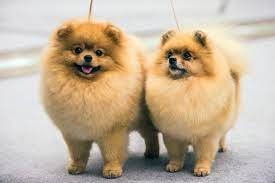
\includegraphics{./figures/dogs.jpeg}
\caption{An example figure}\label{fig:figure1}
}
\end{figure}

\hypertarget{a-subheading-for-the-sake-of-it}{%
\subsection{A subheading for the sake of
it}\label{a-subheading-for-the-sake-of-it}}

We continue writing for no reason. We display a set of figues in
fig.~\ref{fig:subfigures}. Note we can subreference
fig.~\ref{fig:subfigureA} and fig.~\ref{fig:subfigureB}.

\begin{pandoccrossrefsubfigures}

\subfloat[2
dogs]{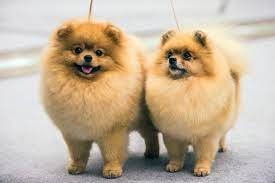
\includegraphics{./figures/dogs.jpeg}\label{fig:subfigureA}}

\subfloat[3
dogs]{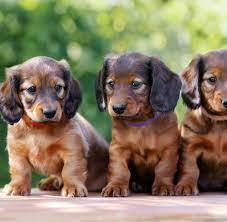
\includegraphics{./figures/dogs2.jpeg}\label{fig:subfigureB}}

\caption[{Overarching subfigure caption}]{Overarching subfigure caption}

\label{fig:subfigures}

\end{pandoccrossrefsubfigures}

\hypertarget{conclusions}{%
\section{Conclusions}\label{conclusions}}

We make some concluding remarks.

\printbibliography[title=References]

\end{document}
